\chapter{Implementace} \label{chap:implementation}
V následující kapitole přistoupíme k popisu prototypu, který jsme v rámci této práce implementovali. Tím navážeme na předchozí kapitolu, ve které jsme řešili návrh systému.\par

\section{Rozsah implementovaného prototypu}
% Jedním z cílů této práce je implementace zvoleného řešení pro vyhledávání pracovníků dle kompetencí na FEL ČVUT.\par
\subsection{Server}
V serverové části prototypu je implementován základní případ užití, tedy UC-1 (\ref{UC1}). Prototyp obsahuje funkční zpracování hexagonální architektury, kterou jsme popsali v předchozí kapitole. Vertikální průřez aplikací je funkční, probíhá synchronní dotaz na funkční datové úložiště s testovacími daty, stejně jako je vidět na sekvenčním digramu (příloha \ref{fig:sequence-synchronous}).\par
% [TODO: nejsou zajištěny ani chybové stavy]
% Popis naimplementované části - neobsahuje AAA (vysvětlit proč), neobsahuje vyhledávání pracovišť (jedná se spíše o POC nikoliv o plnohodnotnou aplikaci), neřeším získávání dat, např. vůbec nejsou přítomny adaptéry aplikační logiky (AAA a jiné vychytávky jako je histrorie hledání apod.), je synchronní přesto, že zvolené řešení by možná vyžadovalo opak, API není kompletní
% Identifikovaná omezení
% - je třeba používat offset, limit, případně prefix, je poměrně pomalé vracet velké množství konceptů
\subsection{Klient}
Klientská část prototypu je přítomna pro demonstraci toho, že komunikace se serverovou částí probíhá a klient je schopný data zpracovávat. V tomto klientu lze vidět implementovanou obdobu W-UC1 (obr. č. \ref{fig:w-uc1}).

\section{Diagram komponent}
% [diagram i s vrstvami (?), možná digram nasazení ]
Diagram komponent konkrétního řešení je k vidění v příloze \ref{fig:component-graphDB}. Jelikož vychází z návrhu zmíněného v minulé kapitole, je obdobou obecného digramu komponent z přílohy \ref{fig:component-model}. V následujících sekcích rozebereme jednotlivé komponenty, technologie, které jsme pro jejich vývoj použili a zmíníme případné ukázky.

\section{Hlavní použité technologie}
V této sekci shrneme základní použité technologie, konkrétnější zástupce poté rozebereme u jednotlivých modulů. Soupis všech použitých technologií je poté připojen v příloze \ref{app:technology-list}.
\subsection{Programovací jazyk pro serverovou část}
Z požadavků specifikovaných v sekci \ref{furps} vyplývá, že použité technologie musí být kompatibilní s budoucím správcem aplikace, což by mělo být některé pracoviště FEL ČVUT. Druhým požadavkem je, aby aplikace byla koncipována jako webová (resp. jako webové rozhraní). V tomto kontextu přichází v úvahu jazyk JAVA, která má na FEL základnu. Variantou by mohlo být nespočet dalších jazyků, které umožňují vývoj webových enterprise aplikací. Jako rozhodující faktor, po požadavcích fakulty, v tomto ohledu vnímáme preference autora samotné aplikace. Jazyk JAVA vyhovuje implementačním dovednostem autora této práce, rozhodli jsme se tedy využít ten. \par
% [TODO: srovnání jazyků?]\par
V rámci jazyka JAVA je možné využít několik různých knihoven pro vývoj webových enterprise aplikací. Pro účely naší práce se mezi sebou příliš neliší.
\paragraph{Některé varianty knihoven:}
\begin{itemize}
    \item Implementace standardu JAVA EE
    \item JAVA Spring (případně jeho nadstavba Spring Boot)
\end{itemize}
V tomto ohledu bereme opět ohledy na preference autora. Zvolili jsme tedy, dnes velmi progresivní, variantu knihovny JAVA Spring, Spring Boot (dokumentace dostupná z: \url{https://spring.io/projects/spring-boot}). Hlavní výhodou Spring Boot je rychlost vývoje za podpory této knihovny a množství kódu, který musí koncový programátor napsat. Tato vlastnost se hodí, hlavně kvůli tomu, že nevyvíjeme kompletní aplikaci, ale prototyp.
% [TODO: srovnání knihoven]
\subsection{Programovací jazyk pro část klient}
Klientská část našeho prototypu bude se serverovou částí komunikovat pomocí REST rozhraní (popsáno níže). Jak jsme zmínili již v úvodu této sekce, klientská aplikace není příliš složitá a je přítomna jen pro demonstraci komunikace se serverem, proto výběr technologie nehraje velkou roli. Zvolili jsme tedy přístup bez jakékoliv další knihovny. Pro klientskou část jsme použili programovací jazyk Javascript, který řeší klientskou logiku, strukturu a vzhled poté řeší HTML a CSS.
\subsection{Databáze}
V kapitole č. \ref{chap:processing} jsme již zmínili příklady různých triple-store databází. Na databázi neklademe žádné speciální požadavky, pouze podporu RDF triplů. Námi zvolená databáze je volně dotupná verze GRAPH-DB (dostupná z: \url{http://graphdb.ontotext.com/}). GRAPH-DB mimojiné používá knihovnu RDF4J, která poskytuje rozhraní jazyku JAVA pro práci s RDF a dalšími přidruženými technologiemi (dokumentace dostupná z: \url{http://rdf4j.org/about/}).
% [TODO: argumentace proč, jsem jí zvolil]
\section{Struktura projektu}
Serverová část prototypu je členěna dle zvolené hexagonální architektury na jednotlivé moduly. V následujících sekcích se zaměříme na popis jednotlivých částí aplikace.
\begin{lstlisting}[caption= Schématicky zobrazená struktura projektu, captionpos=b]
knowledge_search/
|-- application/
    |-- config/
    |-- KnowledgeSearchApplication
|-- domain/
    |-- api/
    |-- logic/
    |-- model/
    |-- spi/
|-- gdb_solution/
    |-- adapters/
    |-- model/
    |-- dao/
|-- rest
    |-- controllers/
    |-- model/
\end{lstlisting} 

\section{Doména}
V diagramu komponent (\ref{fig:component-graphDB}) je doména ve střední části, ve struktuře projektu se nazývá \ctulst(none)!domain!. Doména má čtyři části \ctulst(none)!logic!, \ctulst(none)!model!, \ctulst(none)!spi! a \ctulst(none)!api!.\par
V části \ctulst(none)!logic! se nachází business logika celé aplikace. V nynější verzi se v této vrstvě volají spi repozitáře, složitější logika není přítomna.\par
\noindent Část \ctulst(none)!model! obsahuje doménový model aplikace ve formě rozhraní.
\begin{lstlisting}[language=JAVA, caption= Ukázka rozhraní jedné z entit v doménovém modelu, captionpos=b]
public interface Knowledge extends Identifiable{
    Double getMetric();
    String getInfo();
    <T extends Person> T getOwner();
    <T extends Concept> T getConcept();
}
\end{lstlisting}
Modul \ctulst(none)!spi! obsahuje repozitáře ve formě rozhraní, které později implementuje modul \ctulst(none)!gdb_solution!.
\begin{lstlisting}[language=JAVA, caption= Ukázka rozhraní SPI repozitáře, captionpos=b]
public interface PersonRepository {
    Collection<? extends Knowledge>
    searchPeopleByKnowledge(StringconceptId, int offset, int limit);
    Collection<? extends Person> getAllPersons();
}
\end{lstlisting}
Poslední modul domény je \ctulst(none)!api!, třídy v tomto modulu obsahují rozhraní a implementaci api portů. Tyto porty jsou později používány api adaptéry při volání aplikační logiky.
\section{Spouštěcí modul}
Modul \ctulst(none)!application! má v systému zásadní roli - spouštění a konfigurace aplikace. Spouštění aplikace zajišťuje vstupní bod, třída \ctulst(none)!KnowledgeSearchApplication!. Konfigurace obsahuje adresář \ctulst(none)!config/!. V tomto adresáři jsou definovány tzv. \textit{Spring Bean} třídy, které zajišťují předávání námi zvolené instance určitého objektu Spring IoC kontejneru. Kontejner s instancí dále v běhu aplikace nakládá a vrací jí tam, kde jí potřebujeme.
% [TODO: možná by to chtělo nejaký zdroj] 
V tomto modulu tedy konfigurujeme \textit{Spring Bean} třídy pro všechny ostatní moduly aplikace. Díky tomu máme plnou moc nad tím, kterou implementaci konkrétní části architektury, použijeme. To podporuje náš požadavek na jednoduché změny (viz FURPS+ analýza - \ref{furps}).\par
Mimo výše zmíněného se v této části aplikace nachází další nastavení např. bezpečnostní.
\begin{lstlisting}[language=JAVA, caption= Příklad konfigurace REST kontrolerů, captionpos=b]
@Configuration
public class RestConfiguration {
    @Bean
    public PersonController 
        personController(PersonService personService){
        return new PersonController(personService);
    }

    @Bean
    public ConceptController 
        conceptController(ConceptService conceptService){
        return new ConceptController(conceptService);
    }
}
\end{lstlisting}
\section{API adaptér}
V našem případě se tento modul nazývá \ctulst(none)!rest!, jelikož se jedná o implementaci REST rozhraní. Na diagramu komponent (\ref{fig:component-graphDB}) je tento adaptér k vidění v levé části. Tento modul zprostředkovává komunikaci s klientskou částí prototypu.\par
Ve frameworku \textit{Spring boot} je implementace REST velmi přímočará, je k tomu zapotřebí pouze několik anotací (viz příklad níže). Jedná se o API adaptér, používá tedy API porty implementované v části \ctulst(none)!domain!, v příkladu níže je to například implementace třídy \ctulst(none)!ConceptService!.\par

\begin{lstlisting}[language=JAVA, caption= Příklad REST kontroleru pro operace s koncepty, captionpos=b]
@RestController
@RequestMapping("/concepts")
public class ConceptController {

    private final ConceptService conceptService;

    public ConceptController(ConceptService conceptService) {
        this.conceptService = conceptService;
    }

    @GetMapping("")
    List<ConceptDTO> getAllConcepts() {
        return conceptService.getAllConcepts().stream()
                             .map(ConceptDTO::new)
                             .collect(Collectors.toList());
    }
\end{lstlisting}
V příkladu je navíc vidět, jak jsou koncepty poskytované doménou mapovány na entity vytvořené pro účely klientského použití (anglicky tzv. Data transfer object, zkratka DTO). Toto mapování je zde z toho důvodu, aby nebyla zbytečně přenášena data, která klient nutně nepotřebuje. V našem případě například nepotřebujeme z konceptu nic více než jen název a id. Mapování je v tomto případě jednoduché, je tedy přímo v této třídě. Druhou možností je mít oddělené mapovací třídy.

\section{SPI adaptér}
Klíčovou částí našeho řešení, zajišťující vyhledávání osob dle kompetencí je modul \ctulst(none)!gdb_solution!. Tento modul zajišťuje komunikaci se zvolených datovým uložštěm, v našem případě graphDB. Na diagramu komponent (\ref{fig:component-graphDB}) je tento adaptér k vidění v pravé části.\par
Modul je rozdělen do tří vrstev - \ctulst(none)!adapters!, \ctulst(none)!model! a \ctulst(none)!dao!.
Vrstva \ctulst(none)!adapters! obsahuje implementaci SPI repozitářů, které jsou pomocí rozhraní definovány v doméně. Tyto repozitáře dále využívají třídy vrstvy \ctulst(none)!dao!, která zajišťuje komunikaci s databází.\par
Vrstva \ctulst(none)!dao! obsahuje třídy pro přístup k datům (angicky tzv. data access object). V následující sekci popíšeme, zevrubněji, jak tato vrstva komunikaci s databází zajišťuje.\par
Poslední vrstvou SPI adaptéru je \ctulst(none)!model!, který obsahuje entity. Tyto entity slouží k mapování výsledků databázových dotazů na JAVA objekty. Více se o tomto mapování zmíníme v následující sekci.

\subsection{Přístup k datům}
Jak už jsme výše zmínili, vrstva \ctulst(none)!dao! zodpovídá za komunikaci s databází. Komunikace s GraphDB probíhá pomocí HTTP protokolu a při programovém zpracování této komunikace lze využít dříve zmíněnou knihovnu RDF4J. Mapování výsledků dotazů na vlastní JAVA objekty je poměrně pracné, ostatně proto jsou u relačních databází populární knihovny zajišťující ORM (angl. object-relation mapping) neboli objektově-relační mapování. V našem případě jsme udělali rešerši knihoven podporující OOM neboli ontologicky-relační mapování.
\paragraph{Nalezli jsme následující knihovny:}
\begin{itemize}
    \item Komma (dostupné na: \url{http://komma.enilink.net/docs/framework/objectmapping/index.html})
    \item RDFBeans (dostupné na: \url{https://rdfbeans.github.io/quickstart.html})
    \item JOPA (dostupné na: \url{https://github.com/kbss-cvut/jopa/wiki/})
\end{itemize}
% Další knihovny pro RDF OOMM:
% % https://jena.apache.org/about_jena/contributions.html
% https://www.dataversity.net/empire-rdf-sparql-meet-jpa/#
% http://marmotta.apache.org/sesame.html
Knihovnou, kterou jsme zvolili, je JOPA \cite{JOPA}. Projekt JOPA je, dle repozitáře na github, stále aktivní a shodou okolností je vyvíjen na stejné fakultě, na které vzniká naše práce, FEL ČVUT. V případě problémů bychom tedy mohli jednoduše oslovit tvůrce. Zároveň JOPA umožňuje mapování výsledků dotazů definovaných v \ctulst(none)!dao! (pomocí jazyka SPARQL) na objekty z balíčku \ctulst(none)!gdb_solution/model!, což je přesně to, co potřebujeme.

\begin{lstlisting}[language=JAVA, caption= Příklad definice proměnných polí v entitě PersonGDB za pomoci anotací z knihovny JOPA, captionpos=b]
    @Id
    private URI uri;

    @ParticipationConstraints(nonEmpty = true)
    @OWLDataProperty(iri =
    "http://onto.fel.cvut.cz/koubadom/properties#name")
    private String name;

    @ParticipationConstraints(nonEmpty = true)
    @OWLDataProperty(iri =
    "http://onto.fel.cvut.cz/koubadom/properties#surname")
    private String surname;

    @ParticipationConstraints(nonEmpty = true)
    @OWLDataProperty(iri =
    "http://onto.fel.cvut.cz/koubadom/properties#username")
    private String username;
\end{lstlisting}

\section{Klientská část prototypu}
Klientská část našeho prototypu (na diagramu \ref{fig:component-graphDB} na levé straně) komunikuje se serverovou a demonstruje využitelnost API.\par
Funkční i obsahová stránka klienta není příliš složitá. Součástí klienta je HTML stránka s jednoduchým vyhledávacím polem a tabulkou s výsledkem vyhledávání. Tuto strukturu funkčně obohacuje několik javascriptových tříd. Hlavní funkcí javascriptu je pochopitelně načítaní dat z API, to je realizováno rozhraním funkce \textit{fetch} (dokumentace dostupná na: \url{https://developer.mozilla.org/en-US/docs/Web/API/Fetch_API/Using_Fetch}).
\begin{figure}[htbp!]
	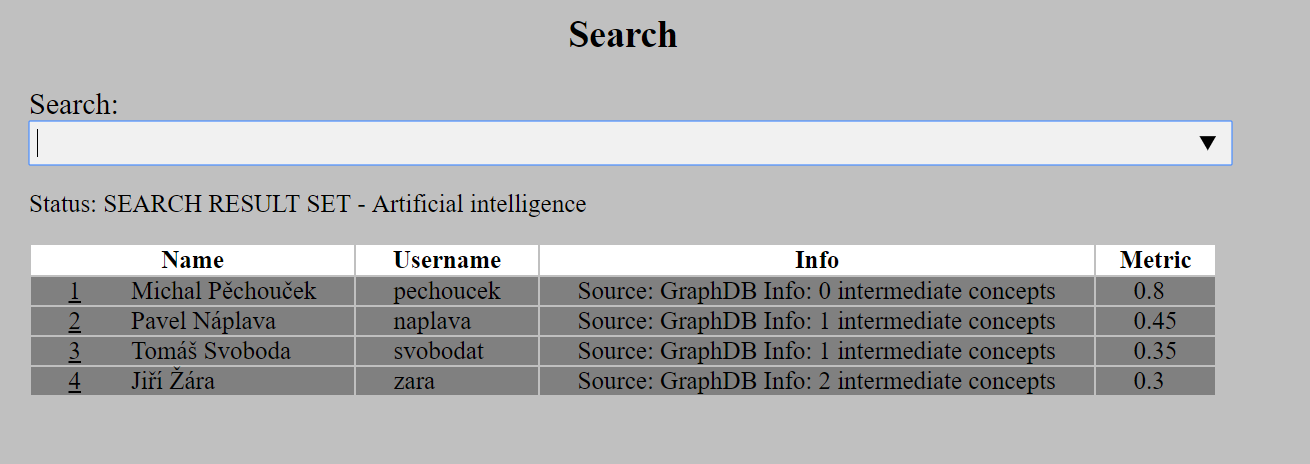
\includegraphics[width=\linewidth]{img/client.png}
	\caption{Snímek klientské části prototypu s načteným výsledkem hledání (zdroj autor)}
	\label{fig:client-screenshot}
\end{figure}

\section{Databáze}
% schema, zmínit mapování na doménový model [TODO možná: doménový model pro naší situaci, pro účely OOM]
Jak jsme zmínili výše, jako triplě-store databázi jsme zvolili GraphDB. V této sekci popíšeme ontologické schéma navržené pro naší databázi.\par
\subsection{Databázové schéma}
Již v kapitole č. \ref{chap:processing} jsme zmínili, že volbu ontologického schematu lze realizovat buď vlastní ontologií, existující ontologií, nebo kombinací obojího.\par
Podrobně naše řešení rozebereme v pozdějších sekcích této kapitoly. Zde však upozorníme na to, k čemu jsme konkrétně použili ontologie. V našem konkrétním řešení používáme ontologii v podstatě jako slovník, ve kterém jsou shromážděny koncepty provázané vazbami. V tomto slovníku poté vyhledáváme koncepty a hlavně jejich souvislosti.\par
Jak jsme již zmínili, tvorba slovníku nebo tezauru je typickým případem užití pro existující ontologii SKOS. Rozhodli jsme se, že pro náš prototyp použijeme tu.\par
Slovník bude obsahovat koncepty, zbývají nám tedy ostatní entity z našeho doménového modelu - znalost, osoba a pracoviště. Tyto budeme ukládat též do ontologií, jelikož toto datové úložiště již máme k dispozici a není třeba zvyšovat komplexnost systému další databází.\par
V příloze \ref{fig:ontology-scheme} je k vidění použité schéma, tzn. původní SKOS schéma (zdroj: \url{https://www.w3.org/2009/08/skos-reference/skos.rdf}) obohacené o další entity (osoba, pracoviště a znalost).
% Pro přehlednost není na obrázku kompletní SKOS schéma.
% [TODO (myslím, že to je pochopitelné a není třeba):Popis: schéma Odkaz na dokumentaci SKOS, krátce popsat entity a vazby]
\subsection{OOM}
Ontologicky-relační mapování probíhá z databáze na entity v balíčku \ctulst(none)!gdb_solution/model!, které jsou implementací rozhraní entit domény z balíčku \ctulst(none)!domain/model!. Tento programový vzor jsme zvolili, jelikož implementace SPI adaptérů se může v čase měnit. Model příslušného řešení tedy musí implementovat rozhraní modelu domény, nicméně může obsahovat další atributy, specifické pro konkrétní řešení. Na obrázku \ref{fig:concept} je celá situace schematicky zobrazena na entitě Koncept. Vidíme, že Koncept z databáze se se mapuje na třídu \ctulst(none)!ConceptGDB! z \ctulst(none)!gdb_solution/model! a s tou dále v \ctulst(none)!domain! pracujeme jako s implementací rozhraní \ctulst(none)!Concept!.
\begin{figure}[htbp!]
	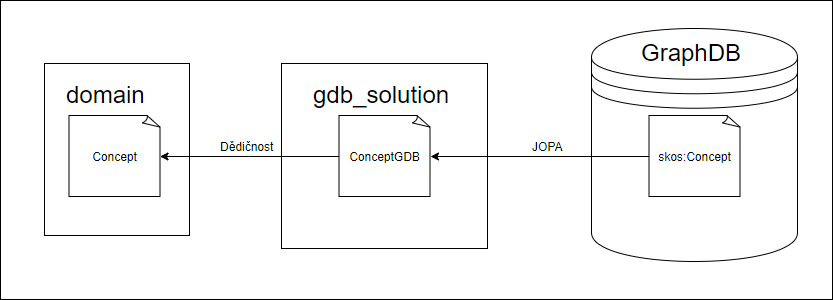
\includegraphics[width=\linewidth]{img/concept.png}
	\caption{Mapování objektů zobrazené schématicky, příklad na objektu Koncept (zdroj autor)}
	\label{fig:concept}
\end{figure}

% \subsubsection{Datový model - ontologie}
% konkrétní diagram tříd, možná schematicky udělat semantickou síť
% Zmínit, že řešení tohoto modulu se může různit, v další kapitole rozebereme naše konkrétní řešení, ale zde zmíníme datový model, ontologický, který použijeme, dá se říct něco o SKOS a alternativách
% Již konkrétní část řešení - konkrétní
% Datový model – návrh ontologie
% Ontologie
% Volba schema databáze
% - varianty SKOS apod. (Denis mi posílal prezentaci), např. http://xmlns.com/foaf/spec/
% - rozšířit SKOS o Person, Knowledge (možná bude potřeba)
% - protege

\section{Popis implementovaného řešení}
Výše jsme rozebrali části, ze kterých se navrhovaný systém skládá. V této sekci rozebereme, v jakých krocích vyhledávání lidí dle kompetencí probíhá a jednotlivé kroky popíšeme.\par
% Před tím než postup rozebereme, je důležité připomenout, že nejdůležitějším požadavek na navrhovaný systém byl požadavek na modularitu (\ref{furps}). Tento požadavek je zde z toho důvodu, že řešený problém je netriviální a je mnoho různých způsobů, jak jej řešit. V následující sekci představíme jedno z možných řešení, jedná se o variantu synchronního průběhu vyhledávání osob dle kompetencí (viz \ref{fig:sequence-synchronous}).\par
\subsection{Jednotlivé kroky vyhledávání}
\begin{enumerate}
    \item \textbf{Seznam konceptů} - klientská část vyšle požadavek na seznam konceptů, na které je možno se dále dotazovat
    \item \textbf{Příjem požadavku a odpověď} - \ctulst(none)!rest! modul požadavek přijme a předá jej \ctulst(none)!domain!, ta poté předá modulu \ctulst(none)!gdb_solution!, který vrací zpět skrz předchozí moduly seznam konceptů s názvem a identifikátorem
    \item \textbf{Vyhledání dle kompetence} - klientská část pošle identifikátor konceptu, pro který je třeba nalézt seznam kompetentních osob
    \item \textbf{Příjem požadavku} - \ctulst(none)!rest! modul požadavek přijme a předá jej \ctulst(none)!domain!, ta poté předá modulu \ctulst(none)!gdb_solution!
    \item \textbf{Zpracování požadavku} - hledaný koncept se využije jako parametr pro použitý databázový dotaz (vysvětleno níže), výsledek dotazu je ještě v komponentě \ctulst(none)!gdb_solution! dále zpracován (vysvětleno níže) a následně vrácen do \ctulst(none)!domain!
    \item \textbf{Návrat dat} - výsledek je vrácen jako seznam osob s vypočtenou sílou znalosti, příklad kompletního výsledku je možno vidět v příloze \ref{app:search-result}
\end{enumerate}

\subsection{SPARQL dotaz}
\subsubsection{Dotaz}
Součástí přílohy \ref{app:sparql-query} je použitý databázový dotaz v jazyce SPARQL. Nejpřímočařejší je popsat dotaz pomocí jeho výsledku. Dotaz vrací výčet konceptů ležících mezi vyhledávaným konceptem a danou osobou a váhu znalosti, kterou osoba k poslednímu z konceptů má. Jako hrana se v tomto průchodu používá relace \textit{semanticRelation}. Tato relace je součástí ontologie SKOS a je nejobecnější vazbou mezi dvěma koncepty, značí, že spolu dva koncepty významově souvisí.\par
Dotaz ve své podstatě prohledává po kružnicích okolí konceptu, ke kterému hledáme znalost, a vyhledává osoby, které se nachází maximálně čtyři \textit{semanticRelation} relace daleko od tohoto konceptu. Číslo čtyři v tomto nemá žádný význam, vzniklo empiricky, jelikož provázanost konceptů přes vazbu \textit{semanticRelation} je tak rozsáhlá, že u pěti již dotaz vrací příliš velký výsledek.
% [Argumentovat použití tohoto dotazu na místo hledán nejkratší cesty]
\subsubsection{Zpracování výsledku dotazu}
Výsledek dotazu je třeba uživateli interpretovat, dotaz vrací sílu znalosti k poslednímu konceptu, který leží mezi osobou a vyhledávaným konceptem, a výčet všech mezilehlých konceptů, neexistuje tedy jednotná metrika, dle které by bylo možné výsledek seřadit. Navíc ve výsledku dotazu se osoby opakují a ve finálním výsledku by se měla každá vyskytovat maximálně jednou.\par
\noindent Výslednou sílu znalosti $W$ jsme vypočítali následujícím vzorcem:
$$W=\frac{w}{n +1}$$
% $$I_K=\sum_{i=1}^{k}\sum_{j=1}^{q}r_i w$$
Kde $w$ je síla znalosti k poslednímu z konceptů a $n$ je počet mezilehlých konceptů.\par
% Vzniklý vzorec není pro naše zkoumání stěžejní, jelikož více než konkrétní výsledky chceme potvrdit, že naše řešení lze využít.\par
Výskyt duplicitních hodnot jsme vyřešili tak, že z celého výsledku bereme pro každou z osob vždy jen záznam s nejvyšším $W$.
% [možná diagram sekvencí - nemusí být]
\section{Rozšiřitelnost}
Z FURPS analýzy (\ref{furps}) vyplývá požadavek na modularitu systému, aby jednotlivé moduly (hlavně \ctulst(none)!gdb_solution!) byly jednoduše nahrazovány jinými implementacemi a podobně.\par
Pokud k takové změně dojde (konkrétně u SPI adaptéru), je třeba implementovat rozhraní potřebných SPI portů. Následně je třeba modifikovat konfiguraci v \ctulst(none)!application! a poskytnout Spring kontejneru příslušné nové implementace SPI adaptérů.
% - největší požadavek
% - ukázat, jak navázat, ukázky kódu
% Rozšiřitelnost projektu a modularita zvoleného řešení
% ukázat na příkladu, jak by šla aplikace rozšířit změnit, jak by se dalo na implementaci navázat
\section{Dokumentace projektu}
Dokumentace implementační části této práce vznikla na několika úrovních:
\begin{itemize}
    \item Javadoc - součástí odevzdaného programu
    \item Dokumentace návrhu a implementačních podrobností - kapitola č. \ref{chap:app-design} a č. \ref{chap:implementation} této práce
    \item Použité knihovny, technologie a nástroje jsou součástí přílohy \ref{app:technology-list}
    % [TODO: součástí příručka - možná]
\end{itemize}
% [TODO: dokumentace API]

\section{Shrnutí}
V této kapitole jsme rozebrali implementační podrobnosti námi realizovaného prototypu systému pro vyhledávání osob dle kompetencí na FEL ČVUT.\par
Prototyp jsme po částech popsali, představili jsme, jak je celý projekt strukturován a připojili jsme i popis technologií. V závěru této kapitoly jsme krok po kroku popsali použitý postup.

% inspirace: https://dspace.cvut.cz/bitstream/handle/10467/24264/F3-DP-2014-Jinoch-Vlastimil-prace.pdf?sequence=3&isAllowed=n

% TripleStore DB:
% https://www.ontotext.com/products/graphdb/editions/ - porovnání edic graphDB (včetně například podpory ellastic search)



%  jednotlivé technologie popsat a citovat, ukázky kódu (nenutit se do toho, je to místy dost strohé), popsat, co na vrstvách má správně probíhat! Technologie - výběr vhodného prostředí - na základě požadavků na program, program stack - frameworks...
